\section{\texorpdfstring{$(2+\epsilon)$}{(2+epsilon)}-Approximate APSP for Weighted Graphs}\label{sec:TZ_2+eps}
Given an undirected, weighted graph $G=(V,E,w)$, our goal is to maintain a $(2+\epsilon)$-approximate all-pair distances in $G$, denoted by $\hat{d}$. 
We provide an algorithm \DynAPSPtwo with parameters $ 0< p,\epsilon\leq 1 $, and $0< \rho \leq 1$ that gives a $(2+\epsilon)$-approximation of APSP for weighted graphs, with ratio between the maximum and minimum weight $W$. Overall, the total update time is $\tilde{O}((pnm + \tfrac{n^2}{p}) \log^2 (nW))$, for an exact statement see Lemma~\ref{lm:mult_time}. The algorithm has constant query time. We provide a high-level algorithm in \Cref{sc:mult_alg}. Then we give further details and parametrized running time analysis of each step in \Cref{sc:mult_time} and the stretch analysis in \Cref{sc:mult_stretch}. In \Cref{sc:mult_result}, we combine these and set the parameter $p$ appropriately to obtain our final result. 
 


    
\subsection{Decremental Data Structures}\label{sc:mult_alg}

We will make use of the $(1+\epsilon_2)$-approximate bunches and clusters that are introduced in \Cref{sc:decr_tools}. However, for efficiency purposes, we do not use these bunches themselves, but instead look at bunches with some additional approximation. The goal is to ensure that the bunches do not increase too often. 

Let $A$ be a set of sampled nodes with a probability $p$. Recall that, for each node $v$, the \emph{pivot} $p(v)$ is the closest node in $A$ to $v$.

Lemma~\ref{lm:approx_bunches_on_G} gives us an approximate pivot $\tilde p(v)$, together with a distance estimate $\dLNbunch$, such that $d_G(v,p(v)) \leq \dLNbunch(v,\tilde{p}(v)) \leq (1+\epsilon_2) d_G(v,p(v))$. Further, we have $(1+\epsilon_2)$-approximate bunches: $\tilde B(v) := \{w\in V : (1+\epsilon_2)d(v,w) < \dLNbunch(v,\tilde p(v))\}$, and distance estimate $\dLNbunch$ such that $d(u,v)\leq \dLNbunch(u,v)\leq (1+\epsilon_2)d(u,v)$ for all $u\in \tilde B(v)$.

%Note that this means we have at any time $t$ that $\tfrac{\dLNbunch^{(t)}(v,\tilde{p}^{(t)}(v))}{1+\epsilon_3}\leq r^{(t)}(v) \leq \dLNbunch^{(t)}(v,\tilde{p}^{(t)}(v))$. Using our guarantee on $\dLNbunch^{(t)}(v,\tilde{p}^{(t)}(v))$, we obtain
% \begin{align*}
%     \tfrac{d^{(t)}(v,p^{(t)}(v))}{1+\epsilon_3}\leq r^{(t)}(v) \leq (1+\epsilon_2)d^{(t)}(v,p^{(t)}(v)).
% \end{align*}\ttodo{check whether this is what we need.}

We now define our final approximate bunch, which we denote by $B(v)$\footnote{In the high-level overview $B(v)$ has been used for the exact bunches. Since exact bunches do not occur in our actual algorithm, $B(v)$ will denote these approximate bunches from here on.}.
\begin{definition}\label{def:app_app_bunch}
We need the following notions related to bunches and clusters:
\begin{itemize}
    \item For all $v \in V$, we keep track of a $(1+\epsilon_3)$-approximate \emph{bunch radius} $r(v)$, which is a $(1+\epsilon_3)$-approximation of the approximate distance to the approximate pivot, i.e., of $\dLNbunch(v,\tilde{p}(v))$. We denote by $r^{(t)}$ the bunch radius at time $t$. Initially, we set $r^{(0)}(v):=\dLNbunch(v,\tilde{p}(v))$. We update $r^{(t)}(v)$ whenever $\dLNbunch(v,\tilde{p}(v)) > (1+\epsilon_3)r^{(t-1)}(v)$, if so then we set $r^{(t)}(v):=\dLNbunch(v,\tilde{p}(v))$.
    \item Initially we set $B^{(0)}(v):= \tilde B^{(0)}(v)$ and whenever $r^{(t)}(v)\neq r^{(t-1)}(v)$ we set $B^{(t)}(v):=\tilde B^{(t)}(v)$.
    \item The \textit{cluster} of a node $u\in V$ is the set $C(u):= \{ v \in V: u \in B(v) \}$.
\end{itemize}    
\end{definition}


 Note that these bunches $B(v)$ increase at most $\log_{1+\epsilon_3}(nW)$ times by construction.
Next, let us investigate the sizes of these sets. 

\begin{lemma}\label{lm:size_heavy}
 At any given time
\begin{enumerate}[(i)]
    \item With high probability, $ A $ has size $\tilde O (p n) $; \label{item:size_A}
    \item With high probability, each bunch $B(v)$ has size $\tilde O (\tfrac{1}{p}) $;  \label{item:size_bunch}
\end{enumerate}
\end{lemma}
\begin{proof}
\begin{enumerate}[(i)]
    \item This follows immediately from the definition of $A$. 
    \item This holds trivially as $B(v)\subseteq \tilde B(v)$, and $|\tilde{B}(v)|=\tilde O(\tfrac{1}{p})$ at any moment in time due to Lemma~\ref{lm:approx_bunches_on_G}.\qedhere
\end{enumerate}
\end{proof}


Now, we give a description of the algorithm, which is a dynamic version of the static algorithm given in the high-level overview, \Cref{sc:high-level_2approx}. Next, we give a proof of correctness and show how to implement each of the steps. We provide a separate initialization procedure, as for some steps it will turn out that the initialization step and the update steps are quite different.\\
Throughout the algorithm, we set $\tilde\delta := (1+\epsilon_4)^{\lceil \log_{1+\epsilon_4}(\delta)\rceil}$ whenever we want a distance estimate $\delta$ to update at most $\log_{1+\epsilon_4}(nW)$ times. Note that we can always maintain such a $\tilde \delta$ with only a constant multiplicative factor in the total update time. Moreover, it is clear that $\delta \leq \tilde \delta \leq (1+\epsilon_4)\delta$.
Below we define the functions \Initialization{}, and functions used after each edge update $\{u,v\}\in E$: \Delete{$u,v$}, \Update{$u,v, w(u,v)$}. Finally we have the \Query{} function that returns a final estimate over different data structures maintained. 
\\ 

\noindent
\textbf{Algorithm} \DynAPSPtwo{$V,E,w,p,\epsilon$}\\
\Initialization{}:

Set $\epsilon_1=\epsilon_2=\epsilon_3=\epsilon_4=\epsilon/3$.
\begin{enumerate}
    \item \textbf{Sampling.} Sample each node with probability $p$ to construct $A$. \label{step:sampling}
    \item \textbf{Distances from $A$.} Compute $(1+\epsilon_1)$-approximate distances $\delta_A(s,v)$ for $s\in A$ and $v\in V$. 
    %Further, for all $v\in V$, initialize a Min-Heap $Q^{\text{dist-from-}A}_v$ that stores the distances $\delta_A(s,v)$ for $s\in A$.
    \item \textbf{Bunches and clusters.} Initialize the algorithm for maintaining the approximate bunches $\tilde B$ and pivots $\tilde p$ according to Lemma~\ref{lm:approx_bunches_on_G}, denoting with $\dLNbunch(v,w)$ the $(1+\epsilon_2)$-approximate distances for $w\in \tilde B(v)$.\\
    Initialize $(1+\epsilon_3)$-approximate bunch radii $r(v)$ with respect to these approximate pivots $\tilde p(v)$.  \label{step:A_MSSP}
    We initialize another approximation to the bunches, denoted by $B(v)$, which will be defined with respect to the bunch radius $r(v)$. Initially, we simply set $B(v)=\tilde{B}(v)$. We let $\delta_B(u,v):=\dLNbunch(u,v)$, and set $\tilde \delta_B(u,v) := (1+\epsilon_4)^{\lceil \log_{1+\epsilon_4}(\delta_B(u,v))\rceil}$. \label{step:bunches}
    \item \textbf{Neighboring bunch data structure.} For $x\in V$ and $v\in V$ such that there exists $y\in N(x)\cap B(v)$ initialize a Min-Heap $Q^{\rm{nbr-bunch}}_{x,v}$, with an entry for \emph{each} $y\in N(x)\cap B(v)$. The key for the Min-Heap is the distance estimate $ \tilde w (x, y) + \tilde\delta_B (y, v) $. Moreover, to make sure the minimal entry, denoted by $\delta^{\rm{nbr-bunch}}(x,v)$, does not change too often, we maintain an additional approximation: $\tilde \delta^{\rm{nbr-bunch}}(x,v):= (1+\epsilon_4)^{\lceil \log_{1+\epsilon_4}(\delta^{\rm{nbr-bunch}}(x,v))\rceil}$. \label{step:init_nbr_bunch}
    \item \textbf{Adjacent data structure.} For $u,v\in V$ initialize a Min-Heap $Q^{\rm{adjacent}}_{u,v}$, with an entry for each $\{u',v'\}\in E$ such that $u'\in B(u)$ and $v' \in B(v)$. The key for the Min-Heap is the distance estimate $\tilde \delta_B(u,u')+\tilde \delta^{\rm{nbr-bunch}}(u',v)$. \label{step:min_heap_nbr} 
\end{enumerate}

\noindent\Delete{$u,v$}:\\
\indent \Update{$u,v,\infty$}\\

\noindent\Update{$u,v,w(u,v)$}:
\begin{enumerate}[(1)]
     \item \textbf{Distances from $A$.} For all $s\in A$, run \Update{$u,v,w(u,v)$} on the SSSP approximation denoted by $\delta_A(s,\cdot)$. %If this leads to a change in $d(s,v')$ for some $v'\in V$ we update the corresponding entry in $Q^{\rm{pivots}}_{v'}$. 
    \item \textbf{Update bunches and heaps.} Maintain the bunches and clusters, and update the heaps accordingly. See below for the details.  \label{step:update3}
\end{enumerate}

 \noindent\Query{$u,v$}:\\
    % \indent Output $\hat d(u,v)$ as follows.
    % \begin{enumerate}[(a)]
    %     \item If $u \in B(v)$ or $v \in B(u)$, set $\hat d(u, v) := \delta_B(v, u)$ or $\hat d(u, v) := \delta_B(u, v)$ respectively. If $u\in B(v)$ and $v\in B(u)$, set $\hat d(u, v) := \min\{\delta_B(v, u), \delta_B(u, v)\}$.
    % \end{enumerate}
    Output $\hat d(u, v)$ to be the minimum of 
    \begin{enumerate}[(a)]\setcounter{enumi}{1}
         \item $\min\{ \dLNbunch(u,\tilde p(u))+\delta_A(v,\tilde p(u)),\delta_A(u,\tilde p(v))+\dLNbunch(v,\tilde p(v))\}$;\label{step:pivot}
        \item The minimum entry of $Q^{\rm{adjacent}}_{u,v}$, which gives $\min\{\tilde \delta_B(u,u')+\tilde \delta^{\rm{nbr-bunch}}(u',v): u'\in B(u)%,\ v'\in B(v),\ (u',v')\in E\text{ and either }u'\in V_{\rm{light}}\text{ or }v'\in V_{\rm{light}}
        \}$. \label{step:nbr_light1}
    \end{enumerate}
    



\paragraph{Update bunches and heaps (Update Step~\ref{step:update3}).}
Now let us look more closely on how we maintain the bunches and clusters, and how these effect the heaps. We maintain the approximate bunches $\tilde B(v)$ for all $v\in V$ by Lemma~\ref{lm:approx_bunches_on_G}. From here maintain the additional approximate bunches $B(v)$ for all $v\in V$ as given in Definition~\ref{def:app_app_bunch}, i.e., 
If there is a change to $\dLNbunch(v',\tilde p(v'))$, do the following two things:\label{step:update_pivots}
    \begin{itemize}
        \item We check if $\dLNbunch^{(t)}(v',\tilde p^{(t)}(v'))> (1+\epsilon_3)r^{(t-1)}(v')$, and if so we set $r^{(t)}(v')=\dLNbunch^{(t)}(v',p^{(t)}(v'))$ and we set $B^{(t)}(v):=\tilde B^{(t)}(v)$. If not, we set $r^{(t)}(v')=r^{(t-1)}(v')$ and $B^{(t)}(v)=B^{(t-1)}(v)$.
    \end{itemize}
 Let $u'\in V$ be a node for which there is a change to the bunch involving a node $w\in V$. Such a change can be: \ref{case:smaller bunch} $w$ can leave the bunch of $u'$ \ref{case:distance in bunch changed} the distance estimate of $w$ to $u'$ can change while $w$ stays within the bunch, or \ref{case:bigger bunch} $w$ can join the bunch of $u'$. We formalize this as follows, using $\Delta$ to denote which case we are in.
    \begin{enumerate}[(i)]
        \item $w\in B^{(t-1)}(u')$ and $w\notin B^{(t)}(u')$, we set $\Delta=\infty$ to indicate that $w$ is no longer in $B(u')$. \label{case:smaller bunch}
        \item $w\in B^{(t-1)}(u')$ and $w\in B^{(t)}(u')$ with an increased distance estimate $\tilde \delta_B^{(t)}(u',w)$, we set $\Delta=\tilde \delta_B^{(t)}(u',w)$ to be the new distance. \label{case:distance in bunch changed}
        \item \label{case:bigger bunch} $w\notin B^{(t-1)}(u')$ and $w\in B^{(t)}(u')$, we set $\Delta=\tilde \delta_B^{(t)}(u',w)$ to be the distance. 
    \end{enumerate}
        
    
    
    Next, we do the following. 
    \begin{itemize}
        \item \UpdateNbrBunchDSBunchChange{$w,u', \infty$} to update the corresponding entries $\tilde w(v',w)+\tilde\delta_B(w,u')$ in the data structures $Q^{\rm{nbr-bunch}}_{v',u'}$ for every $v'\in \text{Set}^{\rm{nbr-bunch}}_{w,u'}$. If this changes the minimal entry $\delta^{\rm{nbr-bunch}}(x,y)$ in $Q^{\rm{nbr-bunch}}_{x,y}$ for some $x,y\in V$, we check whether we need to update $\tilde \delta^{\rm{nbr-bunch}}(x,y)$, if so we run \UpdateAdjacentDSMinHeapChange{$x,y,\tilde \delta^{\rm{nbr-bunch}}(x,y)$}. %The definition and total update time for this function are given in Lemma~\ref{lm:adjacentDS}.
        \item \UpdateAdjacentDS{$w,u',\Delta$} to update the corresponding entries $\tilde\delta_B(u',w)+\tilde\delta^{\rm{nbr-bunch}}(w,v')$ in the data structures $Q^{\rm{adjacent}}_{u',v'}$ for every $v'\in \text{Set}^{\rm{adj-bunch}}_{u',w}$.
    \end{itemize}


\subsection{Further Details and Time Analysis}\label{sc:mult_time}
In this section, we add further details of the procedures described and analyze the total update time. 

\paragraph{Sampling.} Note that $A$ remains unchanged throughout the algorithm, hence it is only sampled once at the initialization. This takes $O(n)$ time. 

\paragraph{Distances from $A$.} We use the decremental shortest path algorithm from Lemma~\ref{lm:decr_MSSP} together with Lemma~\ref{lm:size_heavy}, which bounds the size of $A$, to obtain the following lemma. 

\begin{lemma}\label{lm:A_MSSP}
    With high probability, we can maintain $(1+\epsilon_2)$-approximate SSSP from each node in $A$, providing us with $\delta_A(s,v)$ for $s\in A$ and $v\in V$. We can do this in time $\tilde{O}(pnm)$ if $m=n^{1+\Omega(1)}$ and $pn=n^{\Omega(1)}$, and in time $\tilde O(pn^{1+o(1)}m)$ otherwise.
\end{lemma}
% \begin{proof}
%     % Moreover, we maintain the pivots $p(v)$ by maintaining a Min-Heap $Q^{\rm{pivot}}_v$ for each node $v$, with the distances to all vertices $u\in A$. Additionally, we store the bunch radius for each node $v$, where each time the minimum in the Min-Heap $Q^{\rm{pivot}}_v$ changes, we update the corresponding bunch radius $r(v)$ if $d(v,p(v)) > (1+\epsilon_3)r(v)$. 
% \end{proof}

\paragraph{Bunches and clusters.}
We have approximate bunches $\tilde B(v)$ and pivots $\tilde p(v)$ by Lemma~\ref{lm:approx_bunches_on_G}, now we maintain the bunch radii $r(v)$ and approximate bunches $B(v)$ and clusters $C(v)$ according to Definition~\ref{def:app_app_bunch}. 
As before, we simply set $\tilde \delta_B(u,v):= (1+\epsilon_4)^{\lceil\log_{1+\epsilon_4}(\delta_B(u,v))\rceil}$. It is immediate that these extra steps do not incur more than a constant factor in the running time with respect to Lemma~\ref{lm:approx_bunches_on_G}, so we obtain the following result. 

\begin{lemma}\label{lm:updatebunches}
    We can maintain $(1+\epsilon_3)$-approximate bunch radii $r(v)$ with respect to the approximate pivots $\tilde p$.
    With high probability, we can maintain approximate bunches $B(v)$ and clusters $C(v)$, and distance estimates $\delta_B(v,u)$ for $u\in B(v)$, for all nodes $v\in V$. Moreover, we can maintain $\tilde \delta_B(u,v)$, a $(1+\epsilon_4)$-approximation of $\delta_B(u,v)$ that updates at most $O(\log_{1+\epsilon_4}(nW))$ times. This takes total update time $ \tilde O (\tfrac{mn^\rho}{p}) $, for some arbitrarily small constant $\rho$, if $m=n^{1+\Omega(1)}$, and $\tilde O(\tfrac{mn^{o(1)}}{p})$ otherwise. 
\end{lemma}






\paragraph{Neighboring bunch data structure.} 
To maintain $Q^{\rm{adjacent}}_{u,v}$, we maintain an auxiliary data structure, which is another Min-Heap $Q^{\rm{nbr-bunch}}_{x,v}$. This data structure consists of the following ingredients. We say $B(v)$ is a \emph{neighboring (approximate) bunch} of $x$ if there exists an edge from $x$ to $B(v)$. For every node $ x $, and every neighboring bunch $ B (v) $ our goal is to store  all neighbors $ y $ such that $ y \in B (v) \cap N(x) $ together with $ \tilde w (x, y) + \tilde\delta_B(y, v) $, which allows us to find the neighbor~$ y $ minimizing this sum for each neighboring bunch\footnote{Recall that we denote $\tilde w$ for $(1+\epsilon_4)^{\lceil\log_{1+\epsilon_4}{w}\rceil}$.}. Later, we will combine this with the distance estimate $\tilde\delta_B(u,x)$ for $u\in B(x)$ to get a distance estimate from $u$ to $v$, which will be stored in $Q^{\rm{adjacent}}_{u,v}$. To make sure we do not have to update the entries in $Q^{\rm{adjacent}}_{u,v}$, we do not maintain the minimum of $Q^{\rm{nbr-bunch}}_{x,v}$ exactly, but instead we maintain an additional approximation, denoted $\tilde\delta^{\rm{nbr-bunch}}(x,v)$ that only changes at most a polylogarithmic number of times.

\begin{lemma}\label{lm:NbrBunchDS}
    With high probability, we can maintain the data structures $Q^{\rm{nbr-bunch}}_{x,v}$ for all $x,v\in V$ in total update time $ \tilde O (\tfrac{n^2}{p}\cdot (\log_{1+\epsilon_4}(nW))+\log_{1+\epsilon_3}(nW))) $. Moreover, in the same total update time, we can maintain an approximation $\tilde\delta^{\rm{nbr-bunch}}(x,v)$ of the minimum entry of $Q^{\rm{nbr-bunch}}_{x,v}$ that only changes at most $\log_{1+\epsilon_3}(nW)\log_{1+\epsilon_4}(nW)$ times for each pair $(x,v)$.
\end{lemma}
\begin{proof}
    This data structure is initialized as follows:
    \begin{itemize}
        \item Iterate over every vertex $v\in V$, and over all $y\in B(v)$. Then iterate over all neighbors $x\in N(y)$ of $y$ and add an entry to the data structure $Q^{\rm{nbr-bunch}}_{x,v}$ with key $\tilde{w}(x,y) + \tilde \delta_B(y,v)$.
    
        This takes $ \tilde O (\tfrac{n^2}{p}) $ initialization time, since there are $n$ options for $v$, it has bunch size $\tilde O(\tfrac{1}{p})$, so $\tilde O(\tfrac{1}{p})$ options for $y$, which has at most $n$ neighbors. 
    \end{itemize}
    We need to facilitate two types of updates for an entry of $Q^{\rm{nbr-bunch}}_{x,v}$ corresponding to an edge $\{x,y\}$: increases in the weight $\tilde w(x,y)$ and increases in the distance estimates $\tilde\delta_B(y,v)$. We define the functions \UpdateNbrBunchDSEdgeChange and \UpdateNbrBunchDSBunchChange respectively. 
    
    Next, we consider how to update this data structure. Suppose a value $\tilde\delta_B(y,v)$ changed for some $y\in B(v)$ due to an update to the bunches (Lemma~\ref{lm:updatebunches}), then we would need to change the corresponding entries in $Q^{\rm{nbr-bunch}}_{x,v}$. Lemma~\ref{lm:updatebunches} gives us $y$, $v$, and the new distance $\tilde \delta_B(y,v)$, which we need to update in all data structures $Q^{\rm{nbr-bunch}}_{x,v}$ for which $\{x,y\}\in E$. To do this efficiently, we maintain a set $\text{Set}_{x,y}^{\rm{nbr-bunch-edge}}$ for each edge $\{x,y\}\in E$ that stores for which $v\in V$ there is an entry in $Q^{\rm{nbr-bunch}}_{x,v}$ and a pointer to where in that data structure it appears. We equip this set with the structure of a self-balancing binary search tree, so we have polylogarithmic insertion and removal times. We update this every time the appearance or location in $Q^{\rm{nbr-bunch}}_{x,v}$ changes. Now if $\tilde w(x,y)$ changes due to an update, we can efficiently change the corresponding places in $Q^{\rm{nbr-bunch}}_{x,v}$ for all relevant $v\in V$.
    
    Moreover, for the changes in the distances from the bunches, we maintain a set $\text{Set}_{y,v}^{\rm{nbr-bunch}}$ for each $v\in V, y\in B(v)$ that stores for which $x\in V$ there is an entry in $Q^{\rm{nbr-bunch}}_{x,v}$ and a pointer to where in that data structures it appears. We equip this set with the structure of a self-balancing binary search tree, so we have polylogarithmic insertion and removal times. We update this every time the appearance or location in $Q^{\rm{nbr-bunch}}_{x,v}$ changes. Now if $\tilde\delta_B(y,v)$ changes due to an update, we can efficiently change the corresponding places in $Q^{\rm{nbr-bunch}}_{x,v}$ for all relevant $x\in V$. 
    
    We define the function \UpdateNbrBunchDSEdgeChange{$x,y,\Delta$}, where $\{x,y\}\in E$, and $\Delta$ is the new value $\tilde w^{(t)}(x,y)$, or $\infty$ if the edge $\{x,y\}$ is deleted. Depending on $\Delta$, we do one of the following:
    \begin{enumerate}[(i)]
        \item If $\Delta<\infty$, then we update the corresponding estimates:
        \begin{itemize}
            \item For each entry $v\in \text{Set}_{x,y}^{\rm{nbr-bunch-edge}}$, update the corresponding entry $\tilde w(x,y)+\tilde\delta_B(y,v)$ in $Q^{\rm{nbr-bunch}}_{x,v}$ and update the entry in $\text{Set}_{x,y}^{\rm{nbr-bunch-edge}}$ accordingly.
        \end{itemize}
        \item If $\Delta=\infty$, then we remove the corresponding estimates:
        \begin{itemize}
            \item For each entry $v\in \text{Set}_{x,v}^{\rm{nbr-bunch-edge}}$, remove the corresponding entry in $Q^{\rm{nbr-bunch}}_{x,v}$. 
        \end{itemize}
    \end{enumerate}
    Concerning the total update time of \UpdateNbrBunchDSEdgeChange, we recall that $\tilde w(x,y) = (1+\epsilon_4)^{\lceil \log_{1+\epsilon_4}(w(x,y))\rceil}$. This means that each weight $\tilde w(x,y)$ gets updated at most $\log_{1+\epsilon_4}(W)$ times, giving total update time $\tilde O(\tfrac{n^2}{p}\log_{1+\epsilon_4}(W)$.
    
    We define the function \UpdateNbrBunchDSBunchChange{$y,v,\Delta$}, where $y$ is an element of $B^{(t-1)}(v)$ and/or $B^{(t)}(v)$, and $\Delta$ is the new value $\tilde\delta_B^{(t)}(y,v)$, or $\infty$ if $y$ is no longer in $B(v)$. \UpdateNbrBunchDSBunchChange does one of three things:
    \begin{enumerate}[(i)]
        \item If $\Delta<\infty$, $y\notin B^{(t-1)}(v)$, and $y\in B^{(t)}(v)$, then we add the corresponding new estimates:\label{step:new1}
        \begin{itemize}
            \item We initialize $\text{Set}_{y,v}^{\rm{nbr-bunch}}$ to be empty.
            \item For all neighbors $x\in N(y)$ of $y$, we add $\tilde w(x,y)+\tilde\delta_B(y,v)$ to $Q^{\rm{nbr-bunch}}_{x,v}$ and store $x$ together with its location in $Q^{\rm{nbr-bunch}}_{x,v}$ in $\text{Set}_{y,v}^{\rm{nbr-bunch}}$.
        \end{itemize}
        \item If $\Delta<\infty$, $y\in B^{(t-1)}(v)$, and $y\in B^{(t)}(v)$, then we update the corresponding estimates:\label{step:existing1}
        \begin{itemize}
            \item For each entry $x\in \text{Set}_{y,v}^{\rm{nbr-bunch}}$, update the corresponding entry $\tilde w(x,y)+\tilde\delta_B(y,v)$ in $Q^{\rm{nbr-bunch}}_{x,v}$ and update the entry in $\text{Set}_{y,v}^{\rm{nbr-bunch}}$ accordingly. 
        \end{itemize}
        \item If $\Delta=\infty$, $y\in B^{(t-1)}(v)$, and $y\notin B^{(t)}(v)$, then we remove the corresponding estimates:\label{step:del1}
        \begin{itemize}
            \item For each entry $x\in \text{Set}_{y,v}^{\rm{nbr-bunch}}$, remove the corresponding entries from $Q^{\rm{nbr-bunch}}_{x,v}$ and from $\text{Set}_{y,v}^{\rm{nbr-bunch}}$. 
        \end{itemize}
    \end{enumerate}
    Moreover, if one of these three actions change the minimum of $Q^{\rm{nbr-bunch}}_{x,v}$, this has an impact on the data structures $Q^{\rm{adjacent}}_{\cdot,v}$. We run \UpdateAdjacentDSMinHeapChange{$x,v,\Delta$}, which is defined and analyzed in Lemma~\ref{lm:adjacentDS}, to propagate this change. Here $\Delta$ is the minimum of $Q^{\rm{nbr-bunch}}_{x,v}$. The total update time of \UpdateAdjacentDSMinHeapChange is included in Lemma~\ref{lm:adjacentDS}, and not in this lemma. 
    
    
    As $\tilde\delta_B(y,v)$ can change at most $O(\log_{1+\epsilon_4}(nW))+\log_{1+\epsilon_3}(nW))$ times, and for each time we need at most $\tilde O(\deg(y))=O(n)$ time to update the data structure, we get at most $\tilde O(\deg(y)(\log_{1+\epsilon_4}(nW))+\log_{1+\epsilon_3}(nW)))$ total update time for the pair $(y,v)$. Now note that there are at most $\tilde O(\tfrac{n}{p})$ such pairs, since there are $n$ options for $v$, with $\tilde O(\tfrac{1}{p})$ options for $y\in B(v)$. So we get total update time  $ \tilde O (\tfrac{n^2}{p} \cdot (\log_{1+\epsilon_4}(nW))+\log_{1+\epsilon_3}(nW))) $.
     
    Further, we maintain $\tilde\delta^{\rm{nbr-bunch}}(x,v)$, a $(1+\epsilon_4)$-approximation of the minimal entry $\delta^{\rm{nbr-bunch}}(x,v)$ of $Q^{\rm{nbr-bunch}}_{x,v}$, defined by $\tilde\delta^{\rm{nbr-bunch}}(x,v):= (1+\epsilon_4)^{\lceil\log_{1+\epsilon_4}(\delta^{\rm{nbr-bunch}}(x,v))\rceil}$. 
    Note that $\tilde\delta^{\rm{nbr-bunch}}(x,v)$ is \emph{not} monotone over time, so it is not trivial how often the estimate changes. However, note that $\tilde\delta^{\rm{nbr-bunch}}(x,v)$ increases at most $\log_{1+\epsilon_4}(nW)$ times in a row. It can only decrease $\log_{1+\epsilon_3}(nW)$ times, since the values $\tilde w(x,y)+\tilde\delta_B(y,v)$ are non-decreasing, except if new vertices $y\in B^{(t)}(v)$ are considered. This is only the case when the bunch $B^{(t)}(v)$ grows, which happens at most $\log_{1+\epsilon_3}(nW)$ times by Lemma~\ref{lm:updatebunches}.
\end{proof}

% \begin{remark}
% Note that this data structure gives us a compression of the neighborhood in the following sense:
% Naively, to find out which neighbors of a node $ v $ are contained in which bunches we would have a search space of size $ \sum_{\{u, v\} \in E} | C (v) | $, which by the bound $ | C (v) | \leq \tau $ for light nodes can be reduced to $ \operatorname{deg} {v} \cdot \tau $.
% Note however that this can easily be super-linear in $ n $.
% By restricting ourselves to one relevant (``minimal'') edge per neighboring bunch, we restrict the search space to size $ O (n) $.
% \end{remark}

\paragraph{Adjacent data structure.}
Using $Q^{\rm{nbr-bunch}}_{x,v}$, we construct the required Min-Heap $Q^{\rm{adjacent}}_{u,v}$ for each pair $u,v\in V$. For every pair of nodes $ u, v \in V $ our goal is to store all edges $ \{x, y\} $ such that $ x \in B (u) $ and $ y \in B (v) $, together with the distance $\tilde\delta_B(u,x)+\tilde w(x,y)+\tilde\delta_B(y,v)$.

\begin{lemma}\label{lm:adjacentDS}
    With high probability, we can maintain the data structures $Q^{\rm{adjacent}}_{u,v}$ for all $u,v\in V$ in total update time $ \tilde O (\tfrac{n^2}{p}\log_{1+\epsilon_4}(nW)\log_{1+\epsilon_3}(nW)) $.
\end{lemma}
\begin{proof}

    This data structure is initialized as follows:    
    \begin{itemize}
        \item Iterate over all nodes $ u $, all $ x \in B (u) $, and all neighboring bunches $ B (v) $ of $ x $ and add an entry for $x$ to $Q^{\rm{adjacent}}_{u,v}$ with key $\tilde\delta_B(u,x)+\tilde\delta^{\rm{nbr-bunch}}(x,v)$.
    
    As there are at most $ n $ bunches in total, this takes time $ \tilde O (n \cdot \tfrac{1}{p} \cdot n) = \tilde O (\tfrac{n^2}{ p}) $. 
    \end{itemize}
    Again, we maintain additional data structures to facilitate updates: for each $x,v\in V$, we maintain $\text{Set}_{x,v}^{\rm{adjacent}}$ which shows for which $u\in V$ there is an entry in $Q^{\rm{adjacent}}_{u,v}$ and a pointer to where in that data structure it appears. We update this every time the appearance or location in $Q^{\rm{adjacent}}_{u,v}$ changes. Now if $\tilde\delta_B(u,w)$ changes due to an update, we can efficiently change the corresponding places in $Q^{\rm{adjacent}}_{u,v}$. 
    
    We define the update function \UpdateAdjacentDSBunchChange analogously to the function \UpdateNbrBunchDSBunchChange. \UpdateAdjacentDSBunchChange{$u,x,\Delta$} does one of the following three things:
    \begin{enumerate}[(i)]
        \item If $\Delta<\infty$, $x\notin B^{(t-1)}(u)$, and $x\in B^{(t)}(u)$, then we add the corresponding new estimates:
        \begin{itemize}
            \item We initialize $\text{Set}_{u,x}^{\rm{adj-bunch}}$ to be empty.
            \item For all nodes with non-empty $\tilde\delta^{\rm{nbr-bunch}}(x,v)$, we add $\tilde\delta_B(u,x)+\tilde\delta^{\rm{nbr-bunch}}(x,v)$ to $Q^{\rm{adjacent}}_{u,v}$ and store $v$ together with its location in $Q^{\rm{adjacent}}_{u,v}$ in $\text{Set}_{u,x}^{\rm{adj-bunch}}$.
        \end{itemize}
        \item If $\Delta<\infty$, $x\in B^{(t-1)}(u)$, and $x\in B^{(t)}(u)$, then we update the corresponding estimates:
        \begin{itemize}
            \item For each entry $v\in \text{Set}_{u,x}^{\rm{adj-bunch}}$, update the corresponding entry $\tilde\delta_B(u,x)+\tilde\delta^{\rm{nbr-bunch}}(x,v)$ in $Q^{\rm{adjacent}}_{u,v}$ and update the entry in $\text{Set}_{u,x}^{\rm{adj-bunch}}$ accordingly. 
        \end{itemize}
        \item If $\Delta=\infty$, $x\in B^{(t-1)}(u)$, and $x\notin B^{(t)}(u)$, then we remove the corresponding estimates:
        \begin{itemize}
            \item For each entry $v\in \text{Set}_{u,x}^{\rm{adj-bunch}}$, remove the corresponding entries from $Q^{\rm{adjacent}}_{u,v}$ and from $\text{Set}_{u,x}^{\rm{adj-bunch}}$. 
        \end{itemize}
    \end{enumerate}
    As updates in bunches/distance estimates in bunches happen at most $O(\log_{1+\epsilon_4}(nW)+\log_{1+\epsilon_3}(nW))$ times, see Lemma~\ref{lm:size_heavy}, we get total update time  $ \tilde O (\tfrac{n^2}{p}\cdot (\log_{1+\epsilon_4}(nW)+\log_{1+\epsilon_3}(nW))) $.
    
    We also define the function \UpdateAdjacentDSMinHeapChange to process changes in $\tilde\delta^{\rm{nbr-bunch}}(\cdot,\cdot)$. \UpdateAdjacentDSMinHeapChange{$x,v,\Delta$} does one of the following three things:
     \begin{enumerate}[(i)]
        \item If $\Delta<\infty$ and the distance estimate from $x$ to $v$ is new, then we add the corresponding new estimates:\label{step:new2}
        \begin{itemize}
            \item We initialize $\text{Set}_{x,v}^{\rm{adj-heap}}$ to be empty.
            \item For all $u\in C(x)$, we add $\tilde\delta_B(u,x)+\tilde\delta^{\rm{nbr-bunch}}(x,v)$ to $Q^{\rm{adjacent}}_{u,v}$ and store $u$ together with its location in $Q^{\rm{adjacent}}_{x,v}$ in $\text{Set}_{x,v}^{\rm{adj-heap}}$.
        \end{itemize}
        \item If $\Delta<\infty$ and there already was a distance estimate from $x$ to $v$, then we update the corresponding estimates:\label{step:existing2}
        \begin{itemize}
            \item For each entry $x\in \text{Set}_{x,v}^{\rm{adj-heap}}$, update the corresponding entry $\tilde\delta_B(u,x)+\tilde\delta^{\rm{nbr-bunch}}(x,v)$ in $Q^{\rm{adjacent}}_{u,v}$ and update the entry in $\text{Set}_{x,v}^{\rm{adj-heap}}$ accordingly. 
        \end{itemize}
        \item If $\Delta=\infty$ and there is no longer a distance estimate from $x$ to $v$, then we remove the corresponding estimates:\label{step:del2}
        \begin{itemize}
            \item For each entry $x\in \text{Set}_{x,v}^{\rm{adj-heap}}$, remove the corresponding entries from $Q^{\rm{adjacent}}_{u,v}$ and from $\text{Set}_{x,v}^{\rm{adj-heap}}$. 
        \end{itemize}
    \end{enumerate}
    Since each $\tilde\delta^{\rm{nbr-bunch}}(\cdot,\cdot)$ updates at most $\log_{1+\epsilon_3}(nW)\log_{1+\epsilon_4}(nW)$ times by Lemma~\ref{lm:NbrBunchDS}, we get total update time $\tilde O(\tfrac{n^2}{p}\log_{1+\epsilon_4}(nW))$ for this operation. 

   Together, \UpdateNbrBunchDSBunchChange and \UpdateAdjacentDSBunchChange form the function \UpdateAdjacentDS. To be precise, we define \UpdateAdjacentDS as follows: \\
\UpdateAdjacentDS{$u,v,\Delta$}:
\begin{enumerate}
    \item \UpdateNbrBunchDSBunchChange{$u,v,\Delta$}
    \item \UpdateAdjacentDSBunchChange{$u,v,\Delta$}
\end{enumerate}
This means we obtain total update time $$\tilde O(\tfrac{n^2}{p}(\log_{1+\epsilon_4}(nW)+\log_{1+\epsilon_3}(nW)+\log_{1+\epsilon_3}(nW)\log_{1+\epsilon_4}(nW)))=\tilde O(\tfrac{n^2}{p}\log_{1+\epsilon_4}(nW)\log_{1+\epsilon_3}(nW)).$$
\end{proof}

\paragraph{Query time.}
Finally, we observe that the query is relatively straightforward and can be done in constant time. 

\begin{lemma}
    \DynAPSPtwo has constant query time. 
\end{lemma}
\begin{proof}
    A query $\Query{u,v}$ consists of the minimum over four values. The first two can be computed in constant time, as the components are all maintained explicitly. The last two are maintained explicitly. This gives us constant query time in total. 
\end{proof}



We summarize this section in the following lemma. 

\begin{lemma}\label{lm:mult_time}
    With high probability, the algorithm \DynAPSPtwo has total update time $ \tilde O ((pnm + \tfrac{n^2}{ p})\log^2(nW)) $ if $m=n^{1+\Omega(1)}$, $p=n^{\Omega(1)-1}$, and $m\leq n^{2-\rho}$ for an arbitrarily small constant $\rho$. If $m\geq n^{2-\rho}$, we have total update time $ \tilde O ((pnm + \tfrac{mn^ \rho+n^2}{ p})\log^2(nW)) $. Otherwise we have total running time $ \tilde O ((pnm + \tfrac{n^2}{ p})n^{o(1)}\log^2(nW)) $.
\end{lemma}
\begin{proof}
    We list the total update times as follows:
\begin{itemize}
    \item \textbf{Sampling.} $O(n)$
    \item \textbf{Distances from $A$.}
    \begin{itemize}
	\item $\tilde{O}(pnm)$ if $m=n^{1+\Omega(1)}$ and $pn=n^{\Omega(1)}$
	\item $\tilde O(pn^{1+o(1)}m)$ otherwise.
    \end{itemize}
    \item \textbf{Bunches and clusters.} 
    \begin{itemize}
	\item $ \tilde O (\tfrac{mn^\rho}{p}) $, for some arbitrarily small constant $\rho$, if $m=n^{1+\Omega(1)}$, 
	\item $\tilde O(\tfrac{mn^{o(1)}}{p})$ otherwise.
    \end{itemize}
 %    \item \textbf{Distances from $ V_{\rm{heavy}} $.}
 %    \begin{itemize}
	% \item $ \tilde O (\tfrac{m n }{p\tau}\log_{1+\epsilon_3}(nW)) $ if $m=n^{1+\Omega(1)}$ and $\tfrac{n}{p\tau}=n^{\Omega(1)}$
	% \item $ \tilde O (\tfrac{m n^{1+o(1)} }{p\tau}\log_{1+\epsilon_3}(nW)) $ otherwise.
 %    \end{itemize}
%   \item \textbf{Overlap data structure.}  $\tilde O (\tfrac{n\tau }{p} \cdot\log_{1+\epsilon_3}(nW)\log_{1+\epsilon_4}(nW)) $
   \item \textbf{Neighboring bunch data structure.} $ \tilde O (\tfrac{n^2}{p} (\log_{1+\epsilon_3}(nW)+\log_{1+\epsilon_4}(nW))) $
   \item \textbf{Adjacent data structure.} $ \tilde O (\tfrac{n^2}{p}\log_{1+\epsilon_3}(nW)\log_{1+\epsilon_4}(nW)) $.
\end{itemize}
This means for the case that $m=n^{1+\Omega(1)}$ and $p=n^{\Omega(1)-1}$, we have total update time
$$ \tilde O ((pnm + \tfrac{mn^{\rho}}{p}  + \tfrac{n^2}{ p})\log_{1+\epsilon_3}(nW)\log_{1+\epsilon_4}(nW)) = \tilde O ((pnm + \tfrac{mn^{\rho}}{p} + \tfrac{n^2}{ p})\log^2(nW)), $$
using that we hide constant factors of $1/\epsilon$ in the $\tilde O$-notation. If we furthermore assume that $n^\rho = O(n/p)$, i.e., $p = O(n^{1-\rho})$ for some arbitrarily small $\rho$, then we obtain the simplified version
$$ \tilde O ((pnm +   \tfrac{n^2}{ p})\log^2(nW)).$$
For other choices of $m,n,$ and $p$, we obtain 
$$ \tilde O ((pnm + \tfrac{n^2}{ p})n^{o(1)}\log^2(nW)). $$
\end{proof}



\subsection{Stretch Analysis}\label{sc:mult_stretch}
We can now follow the same structure as outlined in the high-level overview to prove the stretch in different case for each pair $u,v \in V$. In our analysis we also discuss how maintaining approximate bunches and distances impacts the final stretch.

\begin{lemma}\label{lm:mult_stretch}
    For all $u,v\in V$, the distance estimate $\hat{d}(u,v)$ returned by a query to \DynAPSPtwo is a $(2+\epsilon)$-approximation of the distance $d(u,v)$.
\end{lemma}
\begin{proof}
    Let $u,v \in V$. We will show that at any time $t$, if \Query{$u,v$} returns $\hat d^{(t)}(u,v)$, then we have $d^{(t)}(u,v)\leq \hat d^{(t)}(u,v)\leq (2+\epsilon)d^{(t)}(u,v)$. Since we look at all data structures at the same time~$t$, we omit the superscripts $\cdot^{(t)}$ in the remainder of this proof.
    
    First, let us note that $\hat{d}(u,v)$ consists of different distance estimates that all correspond to actual paths in $G$, hence we clearly have $d(u,v)\leq \hat d(u,v)$. Heaps do not contain `old' entries, entries that correspond to paths that are no longer in $G$ at the time of query, since the update functions \UpdateNbrBunchDSBunchChange, \UpdateNbrBunchDSEdgeChange, \UpdateAdjacentDSMinHeapChange, and \UpdateAdjacentDSBunchChange take such entries out as soon as they are no longer relevant. 
    
    Next, we do a case distinction as follows. 
    % Note that these cases are not necessarily distinct, but they are sufficient.
    % \begin{itemize}
    %     \item[Case 1:] $u\in B(v)$ or $v\in B(u)$. \\
    %     Suppose $u\in B(v)$. By Query Step~\ref{step:bunches}, we have $\hat d(u,v)\leq \delta_B(u,v)=\dLNbunch(u,v)\leq (1+\epsilon_2)d(u,v)\leq (1+\epsilon)d(u,v)$. The argument for $v\in B(u)$ is analogous. 
    % \end{itemize}
    Let $\pi$ denote the shortest path from $u$ to $v$.
    
    \begin{figure}[htbp!]
    \centering
    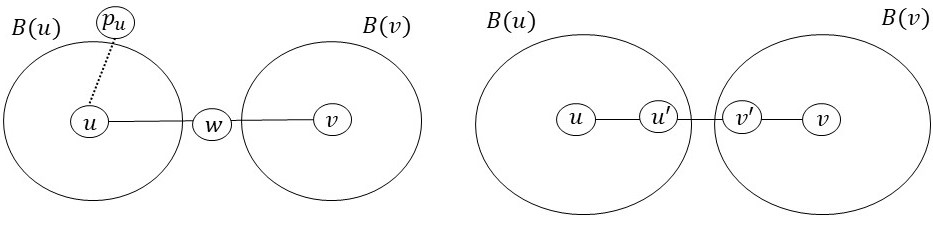
\includegraphics[width=\textwidth]{picture2}
    \caption{Possible scenarios for the overlap between the bunches $B(u)$ and $B(v)$ and the shortest path $\pi$ from $u$ to $v$.}
    \label{fig:pivots2}
    \end{figure}
    
    \begin{itemize}
        \item[Case 1:] There exists $w\in \pi$ such that $w\notin (B(u)\cup B(v))$ (the left case in Figure~\ref{fig:pivots2}).\\
        Since $w\notin B(u)$, we have $d(u,w)\geq   r(u) \geq \tfrac{\dLNbunch(u,\tilde p(u))}{1+\epsilon_3}$, so $\dLNbunch(u,\tilde p(u))\leq (1+\epsilon_3)d(u,w)$. 
        %\geq \tfrac{(1+\epsilon_2)d(v, p(v))}{1+\epsilon_3}$, so $d(v,w) \geq \tfrac{d(v,p(v))}{1+\epsilon_3}$.
        %$d(u,p(u))\leq (1+\epsilon_3)d(u,w)$, 
        Similarly $\dLNbunch(v,\tilde p(v)) \leq (1+\epsilon_3)d(w,v)$. Since $d(u,w)+d(w,v)=d(u,v)$, we have either
        $d(u,w)\leq \tfrac{d(u,v)}{2}$ or $d(v,w)\leq \tfrac{d(u,v)}{2}$. 
        %$d(u,p(u)) \leq (1+\epsilon_3)\tfrac{d(u,v)}{2}$ or $d(v,p(v)) \leq (1+\epsilon_3)\tfrac{d(u,v)}{2}$.
        Without loss of generality, assume $d(u,w) \leq \tfrac{d(u,v)}{2}$, then by Query Step~\ref{step:pivot} in the algorithm we have:
        \begin{align*} 
        \hat{d}(u,v) &\leq \dLNbunch(u,\tilde p(u))+\delta_A(v,\tilde p(u)) \\
        &\leq \dLNbunch(u,\tilde p(u)) +(1+\epsilon_1)d(v,\tilde p(u))\\
        &\leq \dLNbunch(u,\tilde p(u))+(1+\epsilon_1)(d(u,\tilde p(u))+d(u,v))\\
        &\leq \dLNbunch(u,\tilde p(u))+(1+\epsilon_1)(\dLNbunch(u,\tilde p(u))+d(u,v))\\
        &\leq  (2+\epsilon_1)(1+\epsilon_3)d(u,w)+(1+\epsilon_1)d(u,v)\\
        &\leq (2+\tfrac{3}{2}\epsilon_1+\tfrac{1}{2}\epsilon_1\epsilon_3+\epsilon_3)d(u,v)\\
        &\leq (2+\epsilon)d(u,v),
        \end{align*}
        where in the last step we use $\epsilon_1=\epsilon_3=\epsilon/3$.
        \item[Case 2:] 
        There is no $w\in \pi$ such that $w\notin (B(u)\cup B(v))$ (the right case in Figure~\ref{fig:pivots2}).
        \\ 
        This means there has to be a direct edge from the cluster of $u$ to the cluster of $v$: the shortest path $\pi$ consists of a path from $u$ to $u'$, for some $u'\in B(u)$, an edge $\{u',v'\}\in E$, for some $v'\in B(v)$, and a path from $v'$ to $v$ (see the right case in Figure~\ref{fig:pivots2}). Note that in particular this includes the cases where $u\in B(v)$ or $v\in B(u)$, or more general when $B(u)\cap B(v)\neq \emptyset$, since we do not require $u\neq u'$, $v\neq v'$, $u'\notin B(v)$, or $v'\notin B(u)$.\\
        By Query Step~\ref{step:nbr_light1} we have
        \begin{align*}
            \hat d(u,v) &\leq \tilde\delta_B(u,u')+\tilde\delta^{\rm{nbr-bunch}}(u',v)\\
            &\leq (1+\epsilon_4)\delta_B(u,u')+(1+\epsilon_4)\delta^{\rm{nbr-bunch}}(u',v)\\
            &\leq (1+\epsilon_4)(1+\epsilon_2)d(u,u')+(1+\epsilon_4)(\tilde w(u',v')+\tilde\delta_B(v',v))\\ 
            &\leq (1+\epsilon_4)(1+\epsilon_2)d(u,u')+(1+\epsilon_4)^2(w(u',v')+\delta_B(v',v))\\
            &\leq (1+\epsilon_4)(1+\epsilon_2)d(u,u')+(1+\epsilon_4)^2(w(u',v')+(1+\epsilon_2)d(v',v))\\
            &\leq (1+\epsilon_4)^2(1+\epsilon_2)d(u,v)\\
            &\leq (2+\epsilon)d(u,v),
        \end{align*} 
        where in the last step we use $\epsilon_2=\epsilon_4=\epsilon/3$, and $\epsilon<1$. \qedhere
        \end{itemize}

    % \begin{figure}[htbp!]
    % \centering
    % 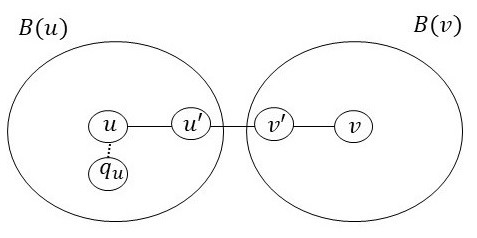
\includegraphics[width=0.5\textwidth]{picture_heavy2}
    % \caption{Possible scenario for the overlap between the bunches $B(u)$ and $B(v)$ and the shortest path $\pi$ from $u$ to $v$ where the estimate can be obtained using heavy pivots $q_u$ and $q_v$.}
    % \label{fig:=heavy_pivots2}
    % \end{figure}
\end{proof}


\subsection{Putting Everything Together}\label{sc:mult_result}
In this section we combine our lemmas in the following theorem. To obtain this result, we pick $p$ to balance the different terms in the total update time.
% \begin{theorem}\label{thm:DynAPSPtwo}
%     Let $G=(V,E)$ be a graph with integer weights bounded by $W$.      
%     The algorithm \DynAPSPtwo{$V,E,w,p,\tau,\rho,\epsilon$} maintains a $(2+\epsilon)$-approximation of APSP, with high probability it has total update time $ \tilde O ((pnm + \tfrac{mn}{p\tau} + m \tau + \tfrac{n^2}{ p})O(\tfrac{\log(nW)}{\epsilon})^{2/\rho+3}) $.
% \end{theorem}

\mainthm*
\begin{proof}
    This follows from Lemma~\ref{lm:mult_time} and~\ref{lm:mult_stretch}, by picking $p$ to minimize $pnm + \tfrac{n^2}{ p}$. This gives $p=\sqrt{\tfrac{n}{m}}$, implying $pnm=\tfrac{n^2}{p}=m^{1/2}n^{3/2}$.
Note that whenever $m=n^{1+\Omega(1)}$ and $m\leq n^{2-\rho}$, this choice of $p$ indeed satisfies the other requirements of Lemma~\ref{lm:mult_time}: $p=n^{\Omega(1)-1}$. When $m=n^{1+o(1)}$, obtain an extra factor $n^{o(1)}$ in the total update time. And when $m\geq n^{2-\rho}$, we obtain the extra factor $n^{\rho}$.
\end{proof}



